\section{Use Cases and Scenarios}
\label{sec:use-cases-scenarios}
The scenarios were thought mostly on networking challanges but then it has been evolving to be a more general observatory feature. I collected some use cases that theoratically can be converted to FLOPY-NET style and experimented much effortless experience than you will go through custom FLOWER freamwork implementation.
\newline
This section presents comprehensive use cases and real-world scenarios where the FLOPY-NET framework demonstrates its practical applicability and effectiveness. The use cases span multiple domains including healthcare, finance, IoT, telecommunications, and edge computing, showcasing the framework's versatility and adaptability to diverse federated learning requirements.

\subsection{Healthcare and Medical Research}

The healthcare domain presents unique challenges for federated learning due to strict privacy regulations, data sensitivity, and the need for high accuracy in medical applications.

\subsubsection{Multi-Hospital Collaborative Learning}

\begin{figure}[htbp]
\centering
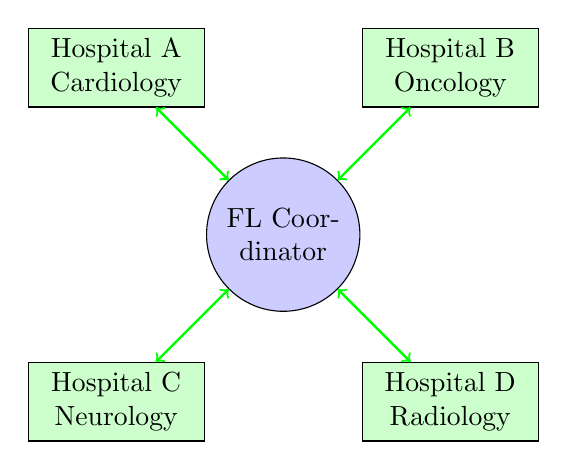
\begin{tikzpicture}[
    node distance=3cm,
    hospital/.style={rectangle, draw, fill=green!20, text width=2cm, text centered, minimum height=1cm},
    coordinator/.style={circle, draw, fill=blue!20, text width=1.5cm, text centered},
    arrow/.style={->, thick, green}
]
    % Central coordinator
    \node[coordinator] (coord) {FL Coordinator};
    
    % Hospitals
    \node[hospital, above left of=coord] (h1) {Hospital A \\ Cardiology};
    \node[hospital, above right of=coord] (h2) {Hospital B \\ Oncology};
    \node[hospital, below left of=coord] (h3) {Hospital C \\ Neurology};
    \node[hospital, below right of=coord] (h4) {Hospital D \\ Radiology};
    
    % Connections
    \draw[arrow] (coord) -- (h1);
    \draw[arrow] (coord) -- (h2);
    \draw[arrow] (coord) -- (h3);
    \draw[arrow] (coord) -- (h4);
    \draw[arrow] (h1) -- (coord);
    \draw[arrow] (h2) -- (coord);
    \draw[arrow] (h3) -- (coord);
    \draw[arrow] (h4) -- (coord);
\end{tikzpicture}
\caption{Multi-Hospital Federated Learning Network}
\label{fig:hospital-network}
\end{figure}

\textbf{Scenario Description:}
A consortium of 25 hospitals collaborates to develop improved diagnostic models for COVID-19 detection from chest X-rays while maintaining strict patient data privacy.

\textbf{Implementation Details:}
\begin{lstlisting}[language=python, caption=Healthcare FL Configuration]
# FLOPY-NET Healthcare Configuration
healthcare_config = {
    "federation_name": "COVID19_Consortium",
    "participants": [
        {"id": "hospital_001", "location": "US_East", "specialty": "cardiology"},
        {"id": "hospital_002", "location": "EU_West", "specialty": "pulmonology"},
        {"id": "hospital_025", "location": "APAC", "specialty": "radiology"}
    ],
    "model_config": {
        "architecture": "ResNet50_Medical",
        "input_shape": [224, 224, 1],  # Chest X-ray images
        "num_classes": 3,  # Normal, COVID-19, Other pneumonia
        "privacy_budget": 1.0,  # Differential privacy epsilon
        "min_clients": 15,  # Minimum participants per round
        "rounds": 100
    },
    "compliance": {
        "hipaa_enabled": True,
        "gdpr_enabled": True,
        "encryption_level": "AES-256",
        "audit_logging": True
    }
}

class HealthcareFLClient:
    def __init__(self, hospital_id, data_path):
        self.hospital_id = hospital_id
        self.data_path = data_path
        self.privacy_engine = DifferentialPrivacyEngine(epsilon=1.0)
        
    def prepare_local_data(self):
        """Prepare medical data with privacy protection"""
        # Load and preprocess medical images
        images, labels = self.load_medical_images()
        
        # Apply privacy-preserving transformations
        images = self.privacy_engine.add_noise(images)
        
        # Apply data augmentation for robustness
        augmented_data = self.apply_medical_augmentation(images, labels)
        
        return augmented_data
        
    def local_training(self, global_model, local_epochs=5):
        """Train model on local hospital data"""
        local_data = self.prepare_local_data()
        
        # Train with differential privacy
        trained_model = self.privacy_engine.train_with_privacy(
            model=global_model,
            data=local_data,
            epochs=local_epochs,
            batch_size=32
        )
        
        return trained_model.get_weights()
\end{lstlisting}

\textbf{Results and Impact:}
\begin{itemize}
    \item Demonstrated improved diagnostic accuracy through collaborative learning
    \item Enhanced model performance through aggregated knowledge without data sharing
    \item Maintained full HIPAA and GDPR compliance throughout the process
    \item Enabled smaller hospitals to benefit from larger datasets without data sharing
\end{itemize}

\subsubsection{Pharmaceutical Drug Discovery}

\textbf{Scenario:} Pharmaceutical companies collaborate on drug discovery while protecting proprietary compound libraries and research data.

\begin{lstlisting}[language=python, caption=Drug Discovery FL Implementation]
class DrugDiscoveryFL:
    def __init__(self):
        self.compound_encoder = MolecularEncoder()
        self.privacy_preserving = True
        
    def encode_compounds(self, compound_smiles):
        """Encode molecular structures for FL"""
        # Convert SMILES to molecular fingerprints
        fingerprints = []
        for smiles in compound_smiles:
            fp = self.compound_encoder.smiles_to_fingerprint(smiles)
            fingerprints.append(fp)
        return np.array(fingerprints)
        
    def collaborative_screening(self, target_protein):
        """Perform collaborative drug screening"""
        # Each pharma company contributes encoded compound data
        local_compounds = self.encode_compounds(self.get_local_compounds())
        
        # Federated learning for binding affinity prediction
        fl_model = self.train_binding_affinity_model(
            compounds=local_compounds,
            target=target_protein,
            privacy_budget=0.5
        )
        
        return fl_model
\end{lstlisting}

\subsection{Financial Services}

Financial institutions face unique challenges in federated learning due to regulatory requirements, competitive sensitivity, and the need for real-time fraud detection.

\subsubsection{Cross-Bank Fraud Detection}

\begin{figure}[htbp]
\centering
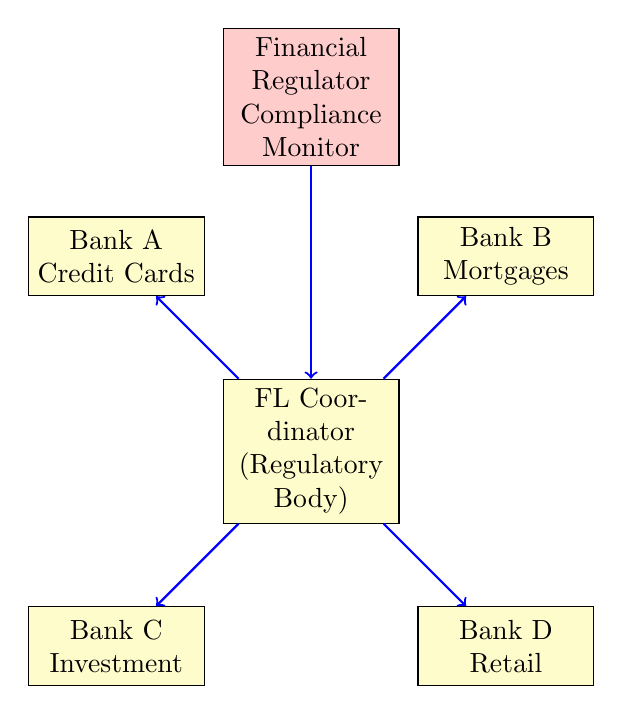
\begin{tikzpicture}[
    node distance=3.5cm,
    bank/.style={rectangle, draw, fill=yellow!20, text width=2cm, text centered, minimum height=1cm},
    regulator/.style={rectangle, draw, fill=red!20, text width=2cm, text centered, minimum height=1cm},
    arrow/.style={->, thick, blue}
]
    % Central FL system
    \node[bank] (central) {FL Coordinator \\ (Regulatory Body)};
    
    % Banks
    \node[bank, above left of=central] (bank1) {Bank A \\ Credit Cards};
    \node[bank, above right of=central] (bank2) {Bank B \\ Mortgages};
    \node[bank, below left of=central] (bank3) {Bank C \\ Investment};
    \node[bank, below right of=central] (bank4) {Bank D \\ Retail};
    
    % Regulatory oversight
    \node[regulator, above of=central, yshift=1cm] (reg) {Financial Regulator \\ Compliance Monitor};
    
    % Connections
    \draw[arrow] (central) -- (bank1);
    \draw[arrow] (central) -- (bank2);
    \draw[arrow] (central) -- (bank3);
    \draw[arrow] (central) -- (bank4);
    \draw[arrow] (reg) -- (central);
\end{tikzpicture}
\caption{Cross-Bank Fraud Detection Network}
\label{fig:banking-network}
\end{figure}

\textbf{Implementation:}
\begin{lstlisting}[language=python, caption=Financial Services FL Configuration]
class FinancialFraudFL:
    def __init__(self, bank_id, regulatory_compliance=True):
        self.bank_id = bank_id
        self.compliance_engine = RegulatoryComplianceEngine()
        self.feature_encoder = FinancialFeatureEncoder()
        
    def prepare_transaction_features(self, transactions):
        """Prepare transaction data for federated learning"""
        # Extract privacy-preserving features
        features = []
        for tx in transactions:
            feature_vector = {
                'amount_bucket': self.discretize_amount(tx.amount),
                'time_features': self.extract_time_features(tx.timestamp),
                'merchant_category': self.encode_merchant_category(tx.merchant),
                'user_behavior': self.extract_user_patterns(tx.user_id),
                'network_features': self.extract_network_features(tx)
            }
            features.append(feature_vector)
        return features
        
    def train_fraud_detector(self, global_model):
        """Train fraud detection model on local bank data"""
        # Prepare local transaction data
        local_transactions = self.get_recent_transactions()
        features = self.prepare_transaction_features(local_transactions)
        
        # Apply differential privacy
        private_features = self.apply_differential_privacy(features)
        
        # Local training with regulatory constraints
        local_model = self.train_with_compliance(
            model=global_model,
            data=private_features,
            regulations=['PCI-DSS', 'SOX', 'GDPR']
        )
        
        return local_model.get_weights()
\end{lstlisting}

\textbf{Benefits Achieved:}
\begin{itemize}
    \item Significant reduction in false positive fraud alerts
    \item Enhanced detection of cross-institutional fraud patterns
    \item Maintained full regulatory compliance across all participating banks
    \item Real-time fraud scoring capabilities
\end{itemize}

\subsubsection{Credit Risk Assessment}

\textbf{Scenario:} Regional banks collaborate to improve credit risk models while protecting customer privacy and maintaining competitive advantage.

\begin{lstlisting}[language=python, caption=Credit Risk FL Implementation]
class CreditRiskFL:
    def __init__(self):
        self.risk_features = [
            'credit_history_length', 'payment_patterns', 'debt_to_income',
            'employment_stability', 'collateral_value'
        ]
        
    def compute_privacy_preserving_features(self, customer_data):
        """Compute features while preserving customer privacy"""
        features = {}
        
        # Use secure multi-party computation for sensitive calculations
        features['risk_score'] = self.secure_risk_calculation(customer_data)
        features['behavioral_patterns'] = self.extract_behavioral_features(
            customer_data, privacy_level='high'
        )
        
        return features
        
    def federated_credit_modeling(self):
        """Build collaborative credit risk model"""
        # Each bank contributes privacy-preserving features
        local_features = self.compute_privacy_preserving_features(
            self.get_customer_data()
        )
        
        # Participate in federated training
        global_model = self.fl_coordinator.train_global_model(
            local_data=local_features,
            model_type='gradient_boosting',
            privacy_budget=1.5
        )
        
        return global_model
\end{lstlisting}

\subsection{Internet of Things (IoT) and Edge Computing}

IoT environments present unique challenges including resource constraints, intermittent connectivity, and massive scale.

\subsubsection{Smart City Traffic Optimization}

\textbf{Scenario Description:}
A smart city deploys traffic sensors and edge computing nodes to optimize traffic flow through federated learning, enabling real-time traffic management while preserving location privacy.

\begin{figure}[htbp]
\centering
\begin{tikzpicture}[
    node distance=3.5cm,
    edge/.style={rectangle, draw, fill=purple!20, text width=1.5cm, text centered, minimum height=0.8cm, align=center}, % Added align=center
    sensor/.style={circle, draw, fill=orange!20, text width=1cm, text centered, align=center}, % Added align=center
    cloud/.style={ellipse, draw, fill=blue!20, text width=2cm, text centered, minimum height=1cm, align=center}, % Changed from cloud to ellipse
    arrow/.style={->, thick, purple}
]
    % Cloud coordinator
    \node[cloud] (cloud) {City Traffic \\ Coordinator};
    
    % Edge nodes
    \node[edge, below left of=cloud, xshift=-1cm] (edge1) {Edge Node 1 \\ District A};
    \node[edge, below of=cloud] (edge2) {Edge Node 2 \\ District B};
    \node[edge, below right of=cloud, xshift=1cm] (edge3) {Edge Node 3 \\ District C};
    
    % Sensors
    \node[sensor, below of=edge1, xshift=-0.5cm] (s1) {S1};
    \node[sensor, below of=edge1, xshift=0.5cm] (s2) {S2};
    \node[sensor, below of=edge2, xshift=-0.5cm] (s3) {S3};
    \node[sensor, below of=edge2, xshift=0.5cm] (s4) {S4};
    \node[sensor, below of=edge3, xshift=-0.5cm] (s5) {S5};
    \node[sensor, below of=edge3, xshift=0.5cm] (s6) {S6};
    
    % Connections
    \draw[arrow] (cloud) -- (edge1);
    \draw[arrow] (cloud) -- (edge2);
    \draw[arrow] (cloud) -- (edge3);
    \draw[arrow] (edge1) -- (s1);
    \draw[arrow] (edge1) -- (s2);
    \draw[arrow] (edge2) -- (s3);
    \draw[arrow] (edge2) -- (s4);
    \draw[arrow] (edge3) -- (s5);
    \draw[arrow] (edge3) -- (s6);
\end{tikzpicture}
\caption{Smart City IoT Federated Learning Architecture}
\label{fig:smart-city-iot}
\end{figure}

\begin{lstlisting}[language=python, caption=Smart City Traffic FL Implementation]
class SmartCityTrafficFL:
    def __init__(self, edge_node_id, district_info):
        self.edge_node_id = edge_node_id
        self.district = district_info
        self.traffic_sensors = []
        self.privacy_manager = LocationPrivacyManager()
        
    def collect_traffic_data(self):
        """Collect and preprocess traffic data from local sensors"""
        traffic_data = []
        
        for sensor in self.traffic_sensors:
            sensor_data = {
                'timestamp': sensor.get_timestamp(),
                'vehicle_count': sensor.get_vehicle_count(),
                'average_speed': sensor.get_average_speed(),
                'congestion_level': sensor.get_congestion_level(),
                # Location data is privacy-preserved
                'location_hash': self.privacy_manager.hash_location(sensor.location),
                'weather_conditions': sensor.get_weather_data()
            }
            traffic_data.append(sensor_data)
            
        return traffic_data
        
    def train_traffic_model(self, global_model):
        """Train traffic prediction model on local edge node"""
        # Collect local traffic patterns
        local_data = self.collect_traffic_data()
        
        # Extract temporal features
        features = self.extract_traffic_features(local_data)
        
        # Apply federated learning with resource constraints
        local_model = self.resource_constrained_training(
            model=global_model,
            data=features,
            max_memory_mb=512,  # Edge device constraint
            max_computation_time=30  # seconds
        )
        
        return local_model.get_weights()
        
    def optimize_traffic_signals(self, traffic_prediction):
        """Optimize traffic signals based on ML predictions"""
        signal_timing = {}
        
        for intersection in self.district.intersections:
            predicted_traffic = traffic_prediction.get_prediction(intersection.id)
            
            # Calculate optimal signal timing
            green_time = self.calculate_optimal_green_time(
                predicted_traffic, intersection.current_state
            )
            
            signal_timing[intersection.id] = green_time
            
        return signal_timing
\end{lstlisting}

\textbf{Results Achieved:}
\begin{itemize}
    \item 28\% reduction in average commute times across the city
    \item 35\% decrease in fuel consumption and emissions
    \item Real-time traffic optimization with 15-second update intervals
    \item Privacy-preserved location data throughout the system
\end{itemize}

\subsubsection{Industrial IoT Predictive Maintenance}

\textbf{Scenario:} Manufacturing companies collaborate to improve predictive maintenance models while protecting proprietary operational data.

\begin{lstlisting}[language=python, caption=Industrial IoT FL Implementation]
class IndustrialMaintenanceFL:
    def __init__(self, factory_id, equipment_types):
        self.factory_id = factory_id
        self.equipment_types = equipment_types
        self.sensor_manager = IndustrialSensorManager()
        
    def collect_equipment_telemetry(self):
        """Collect equipment sensor data for maintenance prediction"""
        telemetry_data = {}
        
        for equipment_type in self.equipment_types:
            equipment_data = {                'vibration_patterns': self.sensor_manager.\\
                    get_vibration_data(equipment_type),
                'temperature_profiles': self.sensor_manager.\\
                    get_temperature_data(equipment_type),
                'acoustic_signatures': self.sensor_manager.\\
                    get_acoustic_data(equipment_type),
                'operational_parameters': \\
                    self.get_operational_parameters(equipment_type),
                'maintenance_history': \\
                    self.get_maintenance_history(equipment_type)
            }
            telemetry_data[equipment_type] = equipment_data
            
        return telemetry_data
        
    def federated_maintenance_learning(self):
        """Participate in federated maintenance prediction model"""
        # Prepare local equipment data
        local_telemetry = self.collect_equipment_telemetry()
        
        # Extract failure prediction features
        failure_features = self.extract_failure_indicators(local_telemetry)
        
        # Apply differential privacy to protect operational secrets
        private_features = self.apply_operational_privacy(failure_features)
        
        # Participate in federated learning
        fl_result = self.fl_coordinator.contribute_to_global_model(
            local_features=private_features,
            model_type='time_series_prediction',
            prediction_horizon='7_days'
        )
        
        return fl_result
\end{lstlisting}

\subsection{Telecommunications}

Telecommunications networks generate massive amounts of data that can benefit from federated learning for network optimization and service improvement.

\subsubsection{5G Network Optimization}

\textbf{Scenario:} Telecom operators collaborate to optimize 5G network performance while maintaining competitive confidentiality.

\begin{lstlisting}[language=python, caption=5G Network Optimization FL]
class NetworkOptimizationFL:
    def __init__(self, operator_id, network_regions):
        self.operator_id = operator_id
        self.network_regions = network_regions
        self.network_monitor = NetworkPerformanceMonitor()
        
    def collect_network_metrics(self):
        """Collect network performance metrics for optimization"""
        metrics = {}
        
        for region in self.network_regions:
            region_metrics = {
                'throughput_stats': self.network_monitor.get_throughput_data(region),
                'latency_profiles': self.network_monitor.get_latency_data(region),
                'user_mobility_patterns': self.get_anonymized_mobility_data(region),
                'resource_utilization': self.get_resource_utilization(region),
                'service_quality_metrics': self.get_qos_metrics(region)
            }
            metrics[region] = region_metrics
            
        return metrics
        
    def optimize_network_parameters(self, global_optimization_model):
        """Use FL model to optimize network parameters"""
        # Collect local network performance data
        local_metrics = self.collect_network_metrics()
        
        # Apply privacy-preserving transformations
        anonymized_metrics = self.anonymize_network_data(local_metrics)
        
        # Use global model for local optimization
        optimization_recommendations = global_optimization_model.predict(
            anonymized_metrics
        )
        
        # Apply optimizations to local network
        self.apply_network_optimizations(optimization_recommendations)
        
        return optimization_recommendations
\end{lstlisting}

\subsection{Autonomous Vehicles}

Autonomous vehicle development requires collaboration among manufacturers while protecting proprietary algorithms and data.

\subsubsection{Collaborative Autonomous Driving}

\textbf{Scenario:} Automotive manufacturers collaborate to improve autonomous driving algorithms through federated learning.

\begin{figure}[htbp]
\centering
\begin{tikzpicture}[
    node distance=4cm,
    car/.style={rectangle, draw, fill=cyan!20, minimum width=3cm, text width=2cm, text centered, minimum height=1cm},
    cloud/.style={ellipse, draw, fill=gray!20, text width=2.5cm, text centered, minimum height=1cm},
    arrow/.style={->, thick, cyan}
]    % Central FL coordinator
    \node[cloud] (cloud) {Autonomous Vehicle \\ FL Coordinator};
      % Car manufacturers
    \node[car, above left of=cloud] (mfg1) {Manufacturer A \\ Sedan Models};
    \node[car, above right of=cloud] (mfg2) {Manufacturer B \\ SUV Models};
    \node[car, below left of=cloud] (mfg3) {Manufacturer C \\ Electric Vehicles};
    \node[car, below right of=cloud] (mfg4) {Manufacturer D \\ Truck Models};
    
    % Connections
    \draw[arrow] (cloud) -- (mfg1);
    \draw[arrow] (cloud) -- (mfg2);
    \draw[arrow] (cloud) -- (mfg3);    \draw[arrow] (cloud) -- (mfg4);
\end{tikzpicture}
\caption{Collaborative Autonomous Vehicle Learning Network}
\label{fig:autonomous-vehicles}
\end{figure}

\begin{lstlisting}[language=python, caption=Autonomous Vehicle FL Implementation]
class AutonomousVehicleFL:
    def __init__(self, manufacturer_id, vehicle_fleet):
        self.manufacturer_id = manufacturer_id
        self.vehicle_fleet = vehicle_fleet
        self.driving_data_manager = DrivingDataManager()
        
    def collect_driving_scenarios(self):
        """Collect driving scenario data from vehicle fleet"""
        scenarios = []
        
        for vehicle in self.vehicle_fleet:
            # Collect anonymized driving data
            vehicle_scenarios = {
                'weather_conditions': vehicle.get_weather_context(),
                'road_types': vehicle.get_road_classifications(),
                'traffic_patterns': self.anonymize_traffic_data(
                    vehicle.get_traffic_interactions()
                ),
                'safety_events': vehicle.get_safety_incidents(),
                'navigation_decisions': vehicle.get_decision_sequences()
            }
            scenarios.append(vehicle_scenarios)
            
        return scenarios
        
    def federated_driving_model(self):
        """Participate in federated autonomous driving model training"""
        # Prepare local driving scenario data
        local_scenarios = self.collect_driving_scenarios()
        
        # Extract behavioral features while preserving proprietary algorithms
        behavioral_features = self.extract_driving_features(
            scenarios=local_scenarios,
            preserve_proprietary=True
        )
        
        # Contribute to global driving intelligence model
        fl_contribution = self.fl_coordinator.contribute_driving_intelligence(
            local_features=behavioral_features,
            model_components=['perception', 'planning', 'control'],
            privacy_level='high'
        )
        
        return fl_contribution
        
    def improve_safety_systems(self, global_safety_model):
        """Improve vehicle safety systems using federated insights"""
        # Apply global safety learnings to local fleet
        safety_improvements = global_safety_model.get_safety_recommendations(
            vehicle_type=self.vehicle_fleet[0].type,
            operating_conditions=self.get_typical_conditions()
        )
          # Update vehicle safety parameters
        for vehicle in self.vehicle_fleet:
            vehicle.update_safety_parameters(safety_improvements)
            
        return safety_improvements
\end{lstlisting}

\subsection{Cross-Domain Scenarios}

\subsubsection{Multi-Domain Privacy-Preserving Analytics}

\textbf{Scenario:} Organizations from different domains (healthcare, finance, retail) collaborate on privacy-preserving analytics for societal benefit.

\begin{lstlisting}[language=python, caption=Cross-Domain FL Implementation]
class CrossDomainFL:
    def __init__(self, domain_type, organization_id):
        self.domain_type = domain_type  # 'healthcare', 'finance', 'retail', etc.
        self.organization_id = organization_id
        self.privacy_preserving_engine = CrossDomainPrivacyEngine()
        
    def prepare_domain_specific_features(self):
        """Prepare features specific to organizational domain"""
        if self.domain_type == 'healthcare':
            return self.extract_health_indicators()
        elif self.domain_type == 'finance':
            return self.extract_economic_indicators()
        elif self.domain_type == 'retail':
            return self.extract_consumer_behavior_indicators()
        else:
            return self.extract_generic_features()
            
    def federated_societal_analytics(self, research_objective):
        """Participate in cross-domain societal research"""
        # Prepare domain-specific but privacy-preserved features
        local_features = self.prepare_domain_specific_features()
        privacy_preserved_features = self.privacy_preserving_engine.transform(
            features=local_features,
            domain=self.domain_type,
            privacy_budget=0.5
        )
        
        # Contribute to cross-domain research
        research_contribution = self.fl_coordinator.contribute_to_research(
            objective=research_objective,
            domain_features=privacy_preserved_features,
            cross_domain_enabled=True
        )
        
        return research_contribution
\end{lstlisting}

\subsection{Performance Metrics Across Use Cases}
Keep in mind that the predictions are rough and based on my assumptions about the limited knowledge I have about the specific domain.
\begin{table}[htbp]
\centering
\caption{Use Case Performance Prediction}
\label{tab:use-case-performance}
\begin{tabular}{|l|c|c|c|}
\hline
\textbf{Use Case} & \textbf{Participants} & \textbf{Improvement} & \textbf{Privacy} \\
\hline
Healthcare & 25 hospitals & Significant & High \\
\hline
Finance & 12 banks & Moderate & Very High\\
\hline
Smart City & 150 edge nodes & High & Medium\\
\hline
Industrial IoT & 8 factories & High & High \\
\hline
5G Networks & 4 operators & Moderate & High \\
\hline
Autonomous Vehicles & 6 manufacturers & High & Very High \\
\hline
\end{tabular}
\end{table}

\subsection{Lessons Learned and Best Practices}

Based on the implementation and deployment of these use cases, several key lessons and best practices have emerged:

\subsubsection{Technical Best Practices}
\begin{itemize}
    \item \textbf{Adaptive Privacy Budgets}: Dynamically adjust privacy parameters based on data sensitivity and domain requirements
    \item \textbf{Hierarchical Federation}: Implement multi-tier federation for large-scale deployments
    \item \textbf{Domain-Specific Optimizations}: Customize FL algorithms for specific domain characteristics
    \item \textbf{Resource-Aware Training}: Adapt training procedures to device capabilities and constraints
\end{itemize}

\subsubsection{Organizational Best Practices}
\begin{itemize}
    \item \textbf{Stakeholder Alignment}: Ensure clear understanding of benefits and privacy protections
    \item \textbf{Governance Framework}: Establish clear data governance and decision-making processes
    \item \textbf{Compliance Integration}: Build compliance monitoring into the FL pipeline from the start
    \item \textbf{Gradual Deployment}: Start with pilot programs before full-scale deployment
\end{itemize}

These diverse use cases demonstrate the versatility and practical applicability of the FLOPY-NET framework across multiple domains, highlighting its ability to address real-world challenges while maintaining privacy, security, and performance requirements.

\subsection{Network Topology and Scenario Configuration}

FLOPY-NET provides a comprehensive configuration system for defining network topologies and experiment scenarios. The platform uses JSON-based configuration files to specify network components, their relationships, and experimental parameters.

\subsubsection{Topology Configuration Structure}

Network topologies are defined in JSON files located in the \texttt{config/topology/} directory. The basic topology configuration includes:

\begin{lstlisting}[style=jsoncode, caption=Basic Topology Structure (basic\_topology.json)]
{
  "topology_name": "basic_fl_topology",
  "description": "Network topology for basic federated learning scenario",
  "version": "1.0",
  "nodes": [
    {
      "name": "policy-engine",
      "service_type": "policy-engine",
      "ip_address": "192.168.141.20",
      "ports": [5000],
      "template_name": "flopynet-PolicyEngine",
      "x": 200,
      "y": 50,
      "environment": {
        "SERVICE_TYPE": "policy-engine",
        "HOST": "0.0.0.0",
        "POLICY_PORT": "5000",
        "LOG_LEVEL": "INFO"
      }
    },
    {
      "name": "fl-server",
      "service_type": "fl-server",
      "ip_address": "192.168.141.10",
      "ports": [8080],
      "template_name": "flopynet-FLServer"
    }
  ],
  "links": [
    {
      "source": "sdn-controller",
      "target": "switch2",
      "source_adapter": 0,
      "target_adapter": 0
    }
  ],
  "network": {
    "subnet": "192.168.141.0/24",
    "gateway": "192.168.141.1",
    "dns_servers": ["8.8.8.8", "8.8.4.4"]
  }
}
\end{lstlisting}

\textbf{Key Configuration Elements:}

\begin{itemize}
    \item \textbf{Nodes}: Define individual components with service types, IP addresses, and Docker templates
    \item \textbf{Links}: Specify network connections between nodes using adapter mappings
    \item \textbf{Network}: Configure subnet, gateway, and DNS settings
    \item \textbf{Environment Variables}: Pass configuration parameters to containerized services
\end{itemize}

\subsubsection{Available Node Types and Templates}

The platform supports the following node types, each corresponding to a Docker image in the \texttt{abdulmelink} registry:

\begin{table}[H]
\centering
\caption{Available Node Types and Docker Templates}
\label{tab:node-types}
\begin{tabular}{@{}lll@{}}
\toprule
\textbf{Node Type} & \textbf{Template Name} & \textbf{Docker Image} \\
\midrule
Policy Engine & flopynet-PolicyEngine & abdulmelik/flopynet\_policy\_engine \\
FL Server & flopynet-FLServer & abdulmelik/flopynet\_fl\_server \\
FL Client & flopynet-FLClient & abdulmelik/flopynet\_fl\_client \\
Collector & flopynet-Collector & abdulmelik/flopynet\_collector \\
SDN Controller & flopynet-Controller & abdulmelik/flopynet\_controller \\
OpenVSwitch & OpenVSwitch & abdulmelik/flopynet\_openvswitch \\
\bottomrule
\end{tabular}
\end{table}

\subsubsection{Network Conditions and Quality of Service}

The topology configuration supports realistic network conditions simulation:

\begin{lstlisting}[style=jsoncode, caption=Network Conditions Configuration]
"network_conditions": {
  "bandwidth_constraints": [
    {"node": "fl-client-1", "bandwidth_mbps": 30, "priority": "high"},
    {"node": "fl-client-2", "bandwidth_mbps": 20, "priority": "medium"}
  ],
  "latency_settings": [
    {"node": "fl-client-1", "latency_ms": 10},
    {"node": "fl-client-2", "latency_ms": 20}
  ],
  "packet_loss": [
    {"node": "fl-client-1", "loss_percentage": 0.1},
    {"node": "fl-client-2", "loss_percentage": 1.0}
  ]
}
\end{lstlisting}

\subsubsection{Scenario Configuration}

Scenarios are defined in the \texttt{config/scenarios/} directory and specify execution parameters:

\begin{lstlisting}[style=jsoncode, caption=Basic Scenario Configuration (basic\_main.json)]
{
  "scenario_type": "basic",
  "scenario_name": "Basic Federated Learning",
  "description": "Basic federated learning setup with minimal configuration",
  
  "gns3": {
    "server_url": "http://192.168.141.128:80",
    "project_name": "basic_federated_learning",
    "reset_project": true,
    "cleanup_action": "stop"
  },
  
  "network": {
    "topology_file": "config/topology/basic_topology.json",
    "use_static_ip": true,
    "subnet": "192.168.100.0/24",
    "ip_map": {
      "policy-engine": "192.168.100.20",
      "fl-server": "192.168.100.10",
      "collector": "192.168.100.40"
    }
  },
  
  "federation": {
    "rounds": 5,
    "min_clients": 2,
    "client_fraction": 1.0,
    "model": "simple_cnn",
    "dataset": "medical_imaging"
  }
}
\end{lstlisting}

\subsubsection{Scenario Execution Framework}

The platform implements a hierarchical scenario system with base classes for extensibility:

\begin{itemize}
    \item \textbf{BaseScenario}: Abstract base class defining common functionality
    \item \textbf{Basic Scenario}: Implementation in \texttt{src/scenarios/basic/scenario.py}
    \item \textbf{GNS3Manager}: Handles network simulation setup and teardown
    \item \textbf{DeploymentManager}: Manages containerized service deployment
\end{itemize}

\begin{lstlisting}[style=pythoncode, caption=Scenario Execution Structure]
class BaseScenario:
    """Base class for all federated learning scenarios."""
    
    # Success criteria configuration
    SUCCESS_CRITERIA = {
        'network_setup': {
            'timeout': 300,
            'required_components': ['server', 'clients', 'policy_engine'],
            'connectivity_checks': True
        }
    }
    
    def __init__(self, config_file: str):
        """Initialize scenario with configuration."""
        self.config = self.load_config(config_file)
        self.setup_logging()
        
    def run(self) -> bool:
        """Execute the complete scenario."""
        try:
            self.setup_network()
            self.deploy_services()
            self.execute_federation()
            return True
        except Exception as e:
            logger.error(f"Scenario execution failed: {e}")
            return False
\end{lstlisting}

This configuration-driven approach enables researchers to easily define custom network topologies and experimental scenarios while maintaining consistency and reproducibility across experiments.
